\documentclass{jsarticle}

% 画像 (SVG 用)
% \usepackage{svg}
\usepackage{float}

% 典型的な数学・フォント類
\usepackage{amsmath}
\usepackage{bm}

% リスティング
\usepackage{listings, jlisting}

% graphicx は dvipdfmx を付けない!(LuaLaTeX なので)
\usepackage[dvipdfmx]{graphicx}

% キャプション
\usepackage[hang,small,bf]{caption}
\usepackage[subrefformat=parens]{subcaption}
\captionsetup{compatibility=false}

\lstset{
  basicstyle={\ttfamily},
  identifierstyle={\small},
  commentstyle={\smallitshape},
  keywordstyle={\small\bfseries},
  ndkeywordstyle={\small},
  stringstyle={\small\ttfamily},
  frame={tb},
  breaklines=true,
  columns=[l]{fullflexible},
  numbers=left,
  xrightmargin=0zw,
  xleftmargin=3zw,
  numberstyle={\scriptsize},
  stepnumber=1,
  numbersep=1zw,
  lineskip=-0.5ex
}
\renewcommand{\lstlistingname}{プログラム}

\title{信号処理II フルレポート(1)}
\author{2022531047 \\中山 涼太}
\begin{document}
\maketitle

\section*{はじめに}
本レポートでは、重み付き最小自乗法(Weighted Least Squares)によるローパスフィルタを設計し、
重み関数に含まれるパラメータ$\alpha, \beta$の設定が、フィルタ特性にどのような影響を与えるかを、複数の重み設定で得られた結果から
比較・考察する。

\section*{課題1}
\begin{quote}
    重み付き最小自乗法による最適なフィルタ係数の導出式を求めよ。
\end{quote}
最小自乗法は自乗誤差が最小となるパラメータを求める問題であり、
式(\ref{original_lsm})で表される計算で処理される。
\begin{gather} \label{original_lsm}
    \min_a E = \int_{-\pi}^{\pi} |W(\omega)(H(\omega)-D(\omega))|^2
\end{gather}
\begin{align*}
    H(\omega) &= a_0 + a_1 e^{-j\omega} + a_2 e^{j2\omega} + \cdots + a_N e^{-jN\omega}\\
    D(\omega) &\text{:所望周波数特性}\\
    W(\omega) &\text{:重み関数}\\
    E&\text{:評価関数}
\end{align*}
ここで、$H(\omega_k)$を次のように行列表現する。
\begin{gather*}
    \bm{a} =
    \begin{bmatrix}
        a_0\quad a_1\quad \cdots \quad a_N
    \end{bmatrix}^t\\
    \bm{q_k} = \begin{bmatrix}
        1\quad e^{j\omega_k}\quad e^{j2\omega_k}\quad \cdots e^{jN\omega_k}
    \end{bmatrix}^t\\
    H(\omega_k) = \bm{q_k}{}^t \bm{a}
\end{gather*}
$\bm{a}$はフィルタ係数を並べたベクトル、$\bm{q_k}$は周波数点$\omega_k$の値を並べたベクトルである。
さらに$\bm{q_k}$を並べたベクトルを$\bm{Q}$とすると、

式(\ref{original_lsm})を次のように行列表現する。
\begin{align}
    E'' = \sum_{k=0}^{L-1}|W(\omega_k) (H(\omega_k) - D(\omega_k))|^2
\end{align}
ここで、$\bm{W}=\text{diag}{W(\omega_k)}, \quad \bm{E} = \bm{W(Qa-d)}$より、
\begin{align}
    E''=(\bm{Qa}-\bm{d})^t \bm{W}^t \bm{W} (\bm{Qa}-\bm{d})
\end{align}
ここで、$\bm{W}=\text{diag}{W(\omega_k)}$は対角行列のため、$\bm{W}=\bm{W}^t$である。したがって、
\begin{align}
    E''&=(\bm{Qa}-\bm{d})^t \bm{W}^2 (\bm{Qa}-\bm{d})\\
    &=\bm{a}^t \bm{Q}^t \bm{W}^2 \bm{Qa} -2\bm{a}^t \bm{Q}^t \bm{W}^2 \bm{d} + \bm{d}^t \bm{W}^2 \bm{d}
\end{align}
と整理できる。$\bm{Q}^t \bm{W}^2 \bm{Q}$が常に対称行列であることより、評価関数を$\bm{a}$で偏微分すると、次の式が得られる。
\begin{align}
    \frac{\partial E''}{\partial \bm{a}} &=
    \begin{bmatrix}
        \frac{\partial E''(\bm{a})}{\partial a_0}\quad \frac{\partial E''(\bm{a})}{\partial a_1\quad}\quad \cdots \frac{\partial E''(\bm{a})}{\partial a_N}
    \end{bmatrix}^t\\
    &= 2\bm{Q}^t \bm{W}^2 \bm{Qa} - 2\bm{Q}^t \bm{W}^2 \bm{d}
\end{align}
これが0となる$\bm{a}$が最小自乗解であるので、$\bm{a}$について整理すると、
\begin{gather}
    2\bm{Q}^t \bm{W}^2 \bm{Qa} - 2\bm{Q}^t \bm{W}^2 \bm{d} = 0\\
    \bm{Q}^t \bm{W}^2 \bm{Qa} - \bm{Q}^t \bm{W}^2 \bm{d} = 0\\
    (\bm{Q}^t \bm{W}^2 \bm{Q})^{-1} \bm{Q}^t \bm{W}^2 \bm{Qa} = (\bm{Q}^t \bm{W}^2 \bm{Q})^{-1} \bm{Q}^t \bm{W}^2 \bm{d}\\
    \bm{a} = (\bm{Q}^t \bm{W}^2 \bm{Q})^{-1} \bm{Q}^t \bm{W}^2 \bm{d}
\end{gather}
となり、$\bm{a}$が求められる。

\section*{課題2}
\begin{quote}
    重み付き最小自乗法によるローパスフィルタの設計プログラムを完成させよ。
\end{quote}
使用したMATLABソースコードを以下のプログラム\ref{wlsm}に示す。

\begin{lstlisting}[caption={重み付き最小自乗法を用いたローパスフィルタ}, label={wlsm}]
clear all; clc; close all

N=24;   % フィルタ係数の数(フィルタ長2N-2)
L=1024; % 周波数サンプル数
dw = pi/(L-1);
wp = 0.25;  % 通過域のエッジ
ws = 0.29;  % 阻止域のエッジ

pe = ceil(wp*L);
se = ceil(ws*L);

d = [ones(pe, 1); zeros(L-pe, 1)];  % 所望特性
Q = [ones(L, 1) cos((0:L-1)'*(1:(N-1))*dw)];    % 規定周波数成分を並べた行列

w = [ones(pe, 1); zeros(se - pe, 1); ones(L - se, 1)]; % 重みベクトル
W = diag(w);    % 重みベクトルを対角成分に持つ対角行列

a = (Q'*W^2*Q)\(Q'*W^2*d);  % 重み付き最小自乗法によるフィルタ係数の推定

coef = [flipud(a(2:end))/2; a(1); a(2:end)/2];  % フィルタ係数の対称性により、長さ2N-2のフィルタ係数を導出

H = fft(coef, 2*L); % 設計したフィルタの周波数特性H
figure(1);
plot(1:length(H(1:L)), abs(H(1:L)), 'LineWidth', 3);
hold on;
plot(1:length(H(1:L)), d, 'LineWidth', 2);
hold off;
\end{lstlisting}

本プログラムでは、通過域・阻止域それぞれに重みを与えるため、重みベクトル$\bm{w}$を構成し、
対角行列$\bm{W}=\text{diag}(\bm{w})$とした。その後、式(11)を用いて、フィルタ係数を算出した。

\section*{課題3}
\begin{quote}
    最小自乗法によるローパスフィルタと、重み付き最小自乗法によるローパスフィルタの結果を比較し、その違いについて報告せよ。また、なぜ設計結果に違いが生じるのか考察せよ。
    ただし、各フィルタは下記の設定で設計すること。
    \begin{itemize}
        \item フィルタ係数の数:$N=24$
        \item 周波数サンプル数:$L=1024$
        \item 通過域のエッジ:$\omega_p=0.25\pi$
        \item 阻止域のエッジ:$\omega_s=\{0.29\pi, 0.32\pi, 0.35\pi\}$
    \end{itemize}
    重み付き最小自乗法による設計のみ、阻止域のエッジを変えたときの結果も報告すること。
\end{quote}
与えられた上記の条件のもと、最小自乗法によるローパスフィルタ(図1)および、重み付き最小自乗法によるローパスフィルタ(図2)を設計した。
\begin{figure}[H]
    \centering
    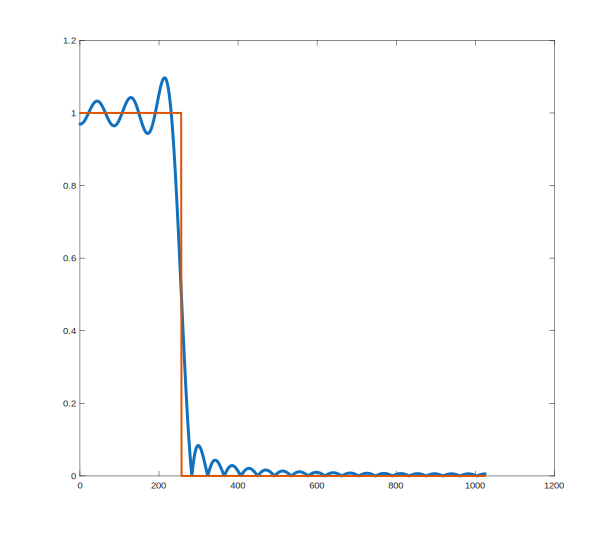
\includegraphics[width=0.4\columnwidth]{img_7_24_0.25.png}
    \caption{最小自乗法によるローパスフィルタ}
\end{figure}
\begin{figure}[H]
    \begin{minipage}[htbp]{0.33\columnwidth}
        \centering
        \includegraphics[width=\columnwidth]{img_report_lp_0.29_1_1.png}
        \subcaption{$\omega_s = 0.29$}
    \end{minipage}
    \begin{minipage}[htbp]{0.33\columnwidth}
        \centering
        \includegraphics[width=\columnwidth]{img_report_lp_0.32_1_1.png}
        \subcaption{$\omega_s = 0.32$}
    \end{minipage}
    \begin{minipage}[htbp]{0.33\columnwidth}
        \centering
        \includegraphics[width=\columnwidth]{img_report_lp_0.35_1_1.png}
        \subcaption{$\omega_s = 0.35$}
    \end{minipage}
    \caption{重み付き最小自乗法によるローパスフィルタ\\$\alpha = 1,\quad\beta = 1$}
\end{figure}
以降、最小自乗法によるローパスフィルタを「甲」、重み付き最小自乗法によるローパスフィルタを「乙」と呼ぶことにする。
% 図1および図2より、乙の方が波形が落ち着いていることが確認できる。
% また、乙の中でも、通過域と阻止域のエッジの間隔が広くなるほど波形の振幅の変化が小さくなり、より滑らかになる傾向が見られる。

% 最小自乗法では、通過域のエッジのみを設定するため、遷移域の設定をしない。そのため、エッジ付近での変化が激しくなり、リップルが目立つ。
% 比較して、重み付き最小自乗法では、通過域や阻止域のエッジ・その帯域での誤差を適切に制御できるため、
% 特定の周波数帯で波形が大きく触れることを抑えることができる。
% また、エッジの間隔(遷移域)が広い場合、フィルタ係数の変化が緩やかに行えるため、波形が安定すると考えられる。

% 以上より、乙は甲に比べ、通過域・阻止域共に波形の安定性が高く、実際の信号処理においても非常に効果を発揮できると言える。
\subsection*{最小自乗法によるローパスフィルタ(甲)の特徴}
図1より、甲では通過域と阻止域の誤差を同等に扱うため、
\begin{itemize}
    \item 通過域・阻止域のリップルが比較的大きい
    \item エッジ付近で波形が激しく振動しやすい
\end{itemize}
といった特徴が見られる。これは、阻止域のエッジを設定しないことにより、遷移域の制御が行えていないためである。
\subsection*{重み付き最小自乗法によるローパスフィルタ(乙)の特徴}
図2(a,b,c)より、乙は甲に比べて明らかに波形が安定している。
特に、阻止域のエッジを変化させた場合でも、波形の振動が抑えられ、フィルタの応答が滑らかである。

これは、乙では通過域・阻止域の誤差に対して任意の重みを付けられるため、指定した帯域の誤差を強く抑えられるためである。
また、エッジ間隔(遷移域)が広いほど、フィルタ係数の変化が緩やかになるため、より平坦な周波数特性になる。

以上より、乙は甲に比べて周波数特性の安定性が高く、より実用的であると言える。

\section*{課題4}
\begin{quote}
    今回作成した重み付き最小自乗法によるローパスフィルタ設計において次式で定義される重み関数の値$\alpha, \beta$を1以外(す
    なわち、 $\alpha, \beta \in (0,1]$)に設定したとき、設計されるフィルタの特
    性がどのように変化するか報告せよ。また、なぜ設計結果に違い
    が生じるのか考察せよ。プログラムをレポートに掲載すること。※設計仕様は、デフォルト設定とする。
    \begin{itemize}
        \item フィルタ係数の数: N=24
        \item 周波数サンプル数: L=1024
        \item 通過域のエッジ: $\omega_p = 0.25\pi$
        \item 阻止域のエッジ: $\omega_s = 0.29\pi$
    \end{itemize}
\end{quote}
\subsection*{重みを変化させた際の観察結果}
今回作成した重み付き最小自乗法によるローパスフィルタ設計において、重み関数の値を1以外にした時のフィルタ特性は以下のように変化することが確認できる。
\begin{figure}[H]
    \centering
    \begin{minipage}[htbp]{0.45\columnwidth}
        \centering
        \includegraphics[width=\columnwidth]{img_report_lp_0.29_0.5_1.png}
        \subcaption{$\alpha = 0.5\quad \beta = 1$}
    \end{minipage}
    \begin{minipage}[htbp]{0.45\columnwidth}
        \centering
        \includegraphics[width=\columnwidth]{img_report_lp_0.29_1_0.5.png}
        \subcaption{$\alpha = 1\quad \beta = 0.5$}
    \end{minipage}
    \caption{重み付き最小自乗法によるローパスフィルタ}
\end{figure}
図3(a)は$\alpha=1, \beta=0.5$での設計結果である。通過域の重みが阻止域の半分であるため、通過域のリップルが図2(a)に比べ増大し、通過域の平坦さが低下している。
一方で、阻止域の減衰性能はほとんど維持されており、阻止域に対する抑制作用は十分であると見受けられる。

図3(b)は$\alpha=0.5, \beta=1$での設計結果である。図3(a)と反対に、阻止域の重みが通過域の半分であるため、阻止域でのリップルが図2(a)に比べ増大し、阻止域の平坦さが低下している。
通過域の平坦さは保たれていると見受けられる。
\begin{figure}[H]
    \centering
    \begin{minipage}[htbp]{0.45\columnwidth}
        \centering
        \includegraphics[width=\columnwidth]{img_report_lp_0.29_0.01_1.png}
        \subcaption{$\alpha = 0.01\quad \beta = 1$}
    \end{minipage}
    \begin{minipage}[htbp]{0.45\columnwidth}
        \centering
        \includegraphics[width=\columnwidth]{img_report_lp_0.29_1_0.01.png}
        \subcaption{$\alpha = 1\quad \beta = 0.01$}
    \end{minipage}
    \caption{重み付き最小自乗法によるローパスフィルタ}
\end{figure}
図4(a)は$\alpha=0.01, \beta=1$での設計結果である。
通過域の重みが極端に小さいため、通過域の特性が著しく劣化している。
一方、阻止域の減衰は良好で、理想的なものであると言える。

図4(b)は$\alpha=1, \beta=0.01$での設計結果である。
図4(a)の特性と真逆で、通過域の平坦さは理想的なものであるが、阻止域の平坦さが低下しており、
減衰性能は著しく悪いといえる。

\begin{figure}[H]
    \centering
    \begin{minipage}[htbp]{0.45\columnwidth}
        \centering
        \includegraphics[width=\columnwidth]{img_report_lp_0.29_0.1_0.2.png}
        \subcaption{$\alpha = 0.1\quad \beta = 0.2$}
    \end{minipage}
    \begin{minipage}[htbp]{0.45\columnwidth}
        \centering
        \includegraphics[width=\columnwidth]{img_report_lp_0.29_0.5_0.5.png}
        \subcaption{$\alpha = 0.5\quad \beta = 0.5$}
    \end{minipage}
    \caption{重み付き最小自乗法によるローパスフィルタ}
\end{figure}

図5(a)は$\alpha=0.1, \beta=0.2$での設計結果である。
図3(a)と比較すると、形状はほとんど等しいと言える。

図5(b)は$\alpha=0.5, \beta=0.5$での設計結果であるが、
こちらについても、図2(a)と同じ形状をしているといえる。

\subsection*{$\alpha, \beta$の関係性}

今回の一連の設計結果から、重み付き最小自乗法によるフィルタの特性は、重み$\alpha, \beta$の絶対値そのものよりも、
その比率$\alpha : \beta$に強く依存すると推測される。
例えば、先の図5(a)と図3(a)は、どちらも$\alpha:\beta = 1:2$であったが、その形状は肉眼で見る限りでは等しいと言える。(以下の再掲を参考にしていただきたい。)
\begin{figure}[H]
    \centering
    \begin{minipage}[htbp]{0.45\columnwidth}
        \centering
        \includegraphics[width=\columnwidth]{img_report_lp_0.29_0.5_1.png}
        \subcaption*{図3 (a)\\$\alpha = 0.5\quad \beta = 1$}
    \end{minipage}
    \begin{minipage}[htbp]{0.45\columnwidth}
        \centering
        \includegraphics[width=\columnwidth]{img_report_lp_0.29_0.1_0.2.png}
        \subcaption*{図5 (a)\\$\alpha = 0.1\quad \beta = 0.2$}
    \end{minipage}
    \caption*{再掲:重み付き最小自乗法によるローパスフィルタ}
\end{figure}
これが数学的に何故かを解明する。

先程の例では、図5(a)の$\alpha, \beta$をそれぞれ5倍すると図3(a)の$\alpha, \beta$と一致する。
そこで、重みベクトル$w$を定数倍することを考える。
\begin{gather}
    \bm{w}' = c\bm{w} (c>0)
\end{gather}
とすると、
\begin{gather}
    \bm{W}' = c\bm{W}\\
    \bm{W}'^2 = c^2 \bm{W}^2
\end{gather}
したがって、新たな$\bm{a}'$は式(11)より
\begin{gather}
    \bm{a}' = (c^2 \bm{Q}^t \bm{W}^2 \bm{Q})^{-1} c^2 \bm{Q}^t \bm{W}^2 \bm{d}\\
    \bm{a}' = \frac{1}{c^2}(\bm{Q}^t \bm{W}^2 \bm{Q})^{-1} c^2 \bm{Q}^t \bm{W}^2 \bm{d} = \bm{a}
\end{gather}
となり、フィルタ係数$\bm{a}$は変化しない。
したがって、重みの絶対値はフィルタ形状に影響せず、通過域と阻止域の重みの比率のみが形状を決定することがわかった。

\subsection*{比率による考察}
改めて$\alpha, \beta$を比率の観点から考察する。

$r=\frac{\alpha}{\beta}$と定義する。
\begin{itemize}
    \item $r=1$のとき\\
    通過域、阻止域の重みが等しいため、どちらの帯域も同等に扱うため、バランスの取れた標準的な形状になる。
    \item $r<1$のとき\\
    通過域は重みが小さいため、誤差が許容されやすくなり、通過域にリップルが顕著に見られるようになる。
    阻止域は重みが大きいため、誤差が許容されにくくなり、阻止域のリップルはほとんど見られなくなる。
    これにより、通過域の安定性は低くなるが、阻止域の減衰性能は向上する。
    \item $r>1$のとき\\
    $r<1$の時と反対に、
    通過域は重みが大きいため、誤差が許容されにくくなり、通過域のリップルは見られなくなる。
    阻止域は重みが小さいため、誤差が許容されやすくなり、阻止域にリップルが顕著に見られるようになる。
    これにより、通過域の平坦性は保たれるが、阻止域の減衰性能は低下する。
\end{itemize}
これらの結果は全て、図3~図5に示される特性と一致していることがわかる。

以下(プログラム2)に重み付き最小自乗法の重みを変化させる仕組みを組み込んだソースコードを掲示する。
\begin{lstlisting}[caption={重み付き最小自乗法を用いたローパスフィルタ}, label={wlsm_lp_wm}]
clear all; clc; close all

N=24;   % フィルタ係数の数(フィルタ長2N-2)
L=1024; % 周波数サンプル数
dw = pi/(L-1);
wp = 0.25;  % 通過域のエッジ
ws = 0.29;  % 阻止域のエッジ

pe = ceil(wp*L);
se = ceil(ws*L);

d = [ones(pe, 1); zeros(L-pe, 1)];  % 所望特性
Q = [ones(L, 1) cos((0:L-1)'*(1:(N-1))*dw)];    % 規定周波数成分を並べた行列

alpha = 0.1;   % 通過域の重み
beta = 1;   % 阻止域の重み
w = [alpha*ones(pe, 1); zeros(se - pe, 1); beta*ones(L - se, 1)]; % 重みベクトル
W = diag(w);    % 重みベクトルを対角成分に持つ対角行列

a = (Q'*W^2*Q)\(Q'*W^2*d);  % 重み付き最小自乗法によるフィルタ係数の推定

coef = [flipud(a(2:end))/2; a(1); a(2:end)/2];  % フィルタ係数の対称性により、長さ2N-2のフィルタ係数を導出

H = fft(coef, 2*L); % Frequency response of the designed filter
figure(1);
plot(1:length(H(1:L)), abs(H(1:L)), 'LineWidth', 3);
hold on;
plot(1:length(H(1:L)), d, 'LineWidth', 2);
hold off;
\end{lstlisting}

\section*{応用課題}
\begin{quote}
    重み付き最小自乗法によるハイパスフィルタの設計のプログラムを完成させよ。
\end{quote}
プログラム2を元に、ハイパスフィルタに変更したソースコードを以下(プログラム3)に示す。
\begin{lstlisting}[caption={重み付き最小自乗法を用いたハイパスフィルタ}, label={wlsm_hp_wm}]
clear all; clc; close all

N=24;   %fixed
L=1024; %fixed
dw = pi/(L-1);
wp = 0.85;  %fixed
ws = 0.82;

pe = ceil(wp*L);
se = ceil(ws*L);

d = [zeros(pe, 1); ones(L-pe, 1)];
Q = [ones(L, 1) cos((0:L-1)'*(1:(N-1))*dw)];

alpha = 0.1;
beta = 1.0;
w = [beta*ones(se, 1); zeros(pe - se, 1); alpha*ones(L - pe, 1)];
W = diag(w);

a = (Q'*W^2*Q)\(Q'*W^2*d);

coef = [flipud(a(2:end))/2; a(1); a(2:end)/2];

H = fft(coef, 2*L);
plot(1:length(H(1:L)), abs(H(1:L)), 'LineWidth', 3);
hold on;
plot(1:length(H(1:L)), d, 'LineWidth', 2);
hold off;
saveas(figure(1), strcat('img_report_hp',"_", num2str(ws),"_",num2str(alpha), "_", num2str(beta),'.png'))
\end{lstlisting}

プログラム3によって作成したハイパスフィルタの周波数特性のグラフを図7に示す。

\begin{figure}[H]
    \centering
    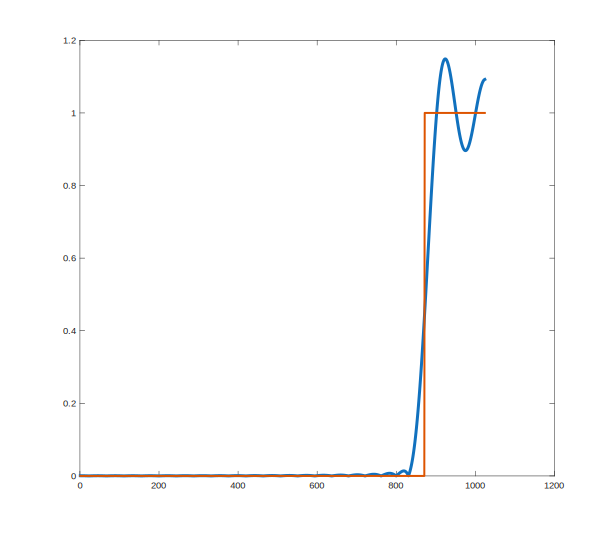
\includegraphics[width=0.4\columnwidth]{img_report_hp_0.82_0.1_1.png}
    \caption{最小自乗法によるハイパスフィルタ\\
    $\alpha=0.1\quad\beta=1$
    }
\end{figure}
\end{document}